\documentclass{article}
\usepackage{tikz}

\begin{document}

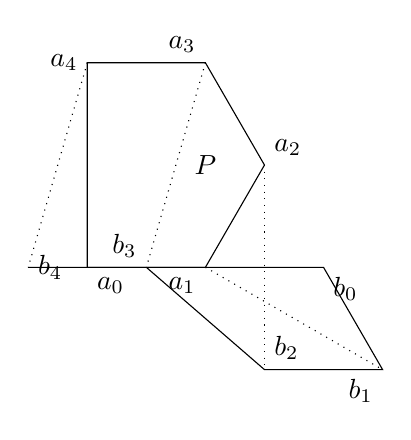
\begin{tikzpicture}[scale=1.5]
    % Define coordinates for the vertices
    \coordinate (a0) at (0, 0);
    \coordinate (a1) at (1, 0);
    \coordinate (a2) at (1.5, 0.866);
    \coordinate (a3) at (1, 1.732);
    \coordinate (a4) at (0, 1.732);
    
    \coordinate (b0) at (2, 0);
    \coordinate (b1) at (2.5, -0.866);
    \coordinate (b2) at (1.5, -0.866);
    \coordinate (b3) at (0.5, 0);
    \coordinate (b4) at (-0.5, 0);

    % Draw the pentagon
    \draw (a0) -- (a1) -- (a2) -- (a3) -- (a4) -- cycle;
    \draw (b0) -- (b1) -- (b2) -- (b3) -- (b4) -- cycle;

    % Draw the dashed lines connecting the vertices of the pentagon to the center
    \draw[dotted] (a0) -- (b0);
    \draw[dotted] (a1) -- (b1);
    \draw[dotted] (a2) -- (b2);
    \draw[dotted] (a3) -- (b3);
    \draw[dotted] (a4) -- (b4);

    % Label the vertices
    \node at (a0) [below right] {$a_0$};
    \node at (a1) [below left] {$a_1$};
    \node at (a2) [above right] {$a_2$};
    \node at (a3) [above left] {$a_3$};
    \node at (a4) [left] {$a_4$};

    \node at (b0) [below right] {$b_0$};
    \node at (b1) [below left] {$b_1$};
    \node at (b2) [above right] {$b_2$};
    \node at (b3) [above left] {$b_3$};
    \node at (b4) [right] {$b_4$};

    % Label the center
    \node at (1, 0.866) {$P$};
\end{tikzpicture}

\end{document}